% ============================================================
% ROTP-PUF-FLASHER : MCyRA 2026 Congress Paper
% Springer CCIS / LLNCS format
% Build prerequisites and steps (see README.md for details):
%   1. Install the Springer class once:  sudo tlmgr install llncs
%      (provides llncs.cls + splncs04.bst; needed on a minimal BasicTeX).
%   2. Build the architecture figure:    pdflatex fig_architecture.tex
%      (produces fig_architecture.pdf, included via \includegraphics).
%   3. Build the paper:  pdflatex main && bibtex main && pdflatex main && pdflatex main
% ============================================================
\documentclass[runningheads]{llncs}

\usepackage[T1]{fontenc}
\usepackage{graphicx}
\usepackage{booktabs}
\usepackage{array}
\usepackage{tabularx}
\usepackage{xcolor}
\usepackage{listings}
\usepackage[expansion=false]{microtype}
\usepackage{amssymb}
\usepackage{hyperref}

\hypersetup{
  colorlinks=true,
  linkcolor=black,
  citecolor=black,
  urlcolor=blue,
  pdftitle={ROTP-PUF-FLASHER: Browser-Based Secure Provisioning and PUF-Bound Encrypted Firmware Execution for ESP32 IoT Devices},
  pdfauthor={Agustin Ahumada Ramirez and Raziel Cesar Campos Sanchez}
}

% Allow long URLs (e.g. the reproducibility link) to break at path separators
\Urlmuskip=0mu plus 1mu\relax
\def\UrlBreaks{\do\/\do-\do.\do:\do?\do=\do\&\do\_}
\urlstyle{rm} % LNCS sample: URLs in roman font, colored by hyperref
\emergencystretch=2em
\hbadness=10000
\vbadness=10000
\hfuzz=11pt

\lstset{
  basicstyle=\ttfamily\small,
  breaklines=true,
  frame=single,
  numbers=left,
  numberstyle=\tiny
}
\AtBeginDocument{\renewcommand{\thelstlisting}{\arabic{lstlisting}}} % Listing 1, not 1.1


\begin{document}


\title{ROTP-PUF-FLASHER: Browser-Based Secure Provisioning and PUF-Bound Encrypted Firmware Execution for ESP32 IoT Devices}

\titlerunning{ROTP-PUF-FLASHER: Secure IoT Provisioning}

\author{Agust\'in Ahumada Ram\'irez\inst{1} \and
        Raziel C\'esar Campos S\'anchez\inst{1}}

\authorrunning{A.~Ahumada Ram\'irez and R.C.~Campos S\'anchez}

\institute{Instituto Nacional de Astrof\'isica, \'Optica y Electr\'onica (INAOE), Tonantzintla, Puebla, M\'exico\\
           \email{contact@agustinahumada.com}}

\maketitle


\begin{abstract}

Provisioning IoT devices without exposing setup material remains an open practical problem: network credentials, server addresses, and device identities are routinely exposed during setup, and firmware modules are typically stored in cleartext on flash. We present ROTP-PUF-FLASHER, a tool that integrates (1)~a browser-based provisioning flow using the Web Serial API to flash the MicroPython base firmware, upload the runtime modules, enroll a runtime SRAM-PUF helper, and store configuration as a PUF-bound encrypted envelope, and (2)~PUF-bound encrypted firmware execution in MicroPython, where, at runtime, a loader in cleartext reconstructs the device's SRAM Physical Unclonable Function (PUF) response, derives a symmetric key via HKDF-SHA256, verifies an HMAC-SHA256 tag over the encrypted module, and decrypts it into RAM for execution, refusing to run on HMAC failure. We map the tool's security properties and remaining gaps to the OWASP IoT Top~10, NIST IR~8259A, and STRIDE, and validate execution, provisioning, and authentication on real ESP32 hardware: identity reconstruction completes in 2.23\,s, secure execution in 2.47\,s, tamper rejection in 2.46\,s, and the encrypted firmware envelope adds 69\,bytes (11.75\%) of overhead over the plaintext module. We further characterize the PUF across three boards, showing near-ideal inter-device distance and cross-device rejection. The open limit is stated explicitly: the configuration and firmware keys depend on the PUF; server-mediated origin is future work.

\keywords{SRAM-PUF \and IoT security \and firmware encryption
  \and MicroPython \and ESP32 \and browser provisioning
  \and OWASP IoT Top~10}
\end{abstract}


\section{Introduction}


Commercial ESP32-class devices are widely deployed in IoT applications but are commonly shipped without activated hardware security controls (eFuses, Secure Boot, or Flash Encryption). Two security weaknesses affect most real-world deployments in this setting.

\emph{Insecure provisioning.}
When a device is set up for the first time, the operator must supply network credentials, server address, and device-specific configuration. Standard practice embeds these in the firmware image or transfers them over an uncontrolled USB or serial connection, leaving them readable to anyone who later inspects the device. To our knowledge, no open-source tool treats this setup as a security-relevant flow backed by a hardware-rooted device identity.

\emph{Unprotected firmware modules.}
Application logic, communication protocols, and credentials stored in MicroPython scripts remain in cleartext on flash, readable and reusable without authorization. Prior work by our group demonstrated the feasibility of HMAC-verified encrypted execution on ESP32/MicroPython~\cite{salinas2026ejecucion}; the present paper extends this into a provisioning tool with browser-based setup and multi-framework security evaluation.

\medskip
\noindent\textbf{Contribution.} We present \textbf{ROTP-PUF-FLASHER}, a tool and evaluation framework with three concrete contributions:

\begin{enumerate}
\item A \emph{browser-based provisioning flow} (the Web Flasher; Web Serial API, Chrome or Edge) that flashes the MicroPython base firmware (\texttt{ESP32\_GENERIC} v1.25.0) with an erase-first policy, uploads the runtime \texttt{.py} modules through the MicroPython raw REPL (read-eval-print loop), enrolls the runtime PUF helper when needed, and writes \texttt{config.json} as a PUF-bound encrypted envelope. \emph{Note:} encrypted payload build remains a host-side CLI step.


\item A \emph{PUF-bound encrypted firmware execution} mechanism in MicroPython: a small loader in cleartext reconstructs the RTC~SLOW SRAM-PUF response (the SRAM in the ESP32 low-power real-time-clock (RTC) domain), derives a symmetric key via HKDF-SHA256, verifies an HMAC-SHA256 tag over the ciphertext, and decrypts the AES-256-CBC payload into RAM for execution. In the demonstrated \texttt{.py} execution path, the protected module is decrypted directly into RAM and is never written to persistent storage in plaintext form.

\item A \emph{multi-framework security evaluation} mapping the tool's security properties against the OWASP IoT Top~10~\cite{owasp2018iot}, NIST IR~8259A~\cite{nist8259a}, and STRIDE~\cite{shostack2014threat}, with measured performance results on real hardware.
\end{enumerate}

\noindent\textbf{Open problem (stated explicitly).}
The decryption key is derived exclusively from the PUF. An adversary who reconstructs the PUF, which is possible on a device without Secure Boot if the boot path is physically replaced, obtains the same key. Moreover, during provisioning and MicroPython execution the browser or host obtains derived key material to build encrypted artifacts. The architecturally correct solution requires server participation in key and configuration origin; Sect.~\ref{sec:discussion} details this limit, which is reserved for thesis/journal work, not claimed here.

\medskip
The rest of the paper reviews background and related work (Sect.~\ref{sec:background}), describes the threat model and design (Sect.~\ref{sec:architecture}), details the implementation (Sect.~\ref{sec:implementation}), presents the security and performance evaluations (Sects.~\ref{sec:security} and~\ref{sec:performance}), and closes with limitations and conclusions (Sects.~\ref{sec:discussion} and~\ref{sec:conclusion}).


\section{Background and Related Work}
\label{sec:background}


\subsection{SRAM Physical Unclonable Functions}

SRAM cells power up to a manufacturing-determined preferred state, a unique and reproducible fingerprint~\cite{holcomb2009powerup} that must be stable enough to reproduce on the same chip yet differ across chips to prevent transplantation~\cite{gao2020puf}. Because SRAM responses are noisy, reliable key derivation requires error correction via a fuzzy extractor or helper-data mechanism~\cite{dodis2008fuzzy}. Peer-reviewed reliability studies show that stability depends on cell selection policy, operating conditions, aging, and spatial correlation~\cite{baturone2015improved,saraza2021improving,wilde2018spatial}. Remanence-based side-channel attacks on SRAM PUFs have been demonstrated~\cite{zeitouni2016remanence}; we treat remanence decay as a real attack surface and do not claim resistance to cold-boot, timed power-down, or semi-invasive capture.

On ESP32, Stan\'{i}\v{c}ek's \texttt{esp32\_puflib}~\cite{stanicek2022esp32puflib} provides enrollment, helper-data generation, and reconstruction targeting the RTC~FAST SRAM and deep-sleep DATA~SRAM. Our MicroPython adaptation targets \emph{RTC~SLOW} SRAM, the surface reachable by runtime register cycling under MicroPython (RTC~FAST and deep-sleep DATA~SRAM remain future work); this constrains it to laboratory control status and does not claim native \texttt{esp32\_puflib} compatibility.

\subsection{Encrypted Firmware Distribution}

The IETF SUIT manifest model~\cite{rfc9124_suit} authenticates firmware metadata, versioning, and payload digests for constrained devices; that update-delivery layer is complementary to this paper rather than a claimed contribution. Our focus is narrower: protecting selected MicroPython firmware modules with a PUF-derived key reconstructed on demand. Espressif's \texttt{esp\_encrypted\_img}~\cite{espressif_esp_encrypted_img}, the closest official reference, supports ECIES-P256 but still depends on a device secret in eFuse or firmware, which this reversible (no-eFuse) design avoids. The broader IoT attestation literature supports hardware-rooted checking~\cite{kuang2022survey} but targets attestation services rather than PUF-bound encrypted execution.

\subsection{Related Work}
\label{sec:sota}

Table~\ref{tab:sota} compares representative work on secure firmware update, PUF-bound update or integrity, OS-level PUF support, blockchain-assisted update, and browser-device provisioning. These works address pieces of the problem, but none of the surveyed systems combines browser-based provisioning with PUF-bound encrypted firmware execution on ESP32/MicroPython or evaluates the implementation against OWASP IoT Top~10, NIST IR~8259A, and STRIDE.

\begin{table*}[t]
\caption{Comparison with related works. FW prot./PUF: firmware update, integrity, code dissemination, or execution protection, with PUF binding indicated where applicable. Browser prov.: browser-based interface used for provisioning or flashing. OWASP/NIST/STRIDE: simultaneous evaluation against all three frameworks.}
\label{tab:sota}
\centering\footnotesize
\setlength{\tabcolsep}{3pt}
\newcolumntype{L}[1]{>{\raggedright\arraybackslash}p{#1}}
\resizebox{\linewidth}{!}{%
\begin{tabular}{L{3.2cm}lccc}
\toprule
\textbf{Work} & \textbf{Hardware} & \textbf{FW prot.} & \textbf{Browser} & \textbf{OWASP/} \\
 \textbf{(Year)} & \textbf{Platform} & \textbf{/ PUF binding} & \textbf{provisioning} & \textbf{NIST/STRIDE} \\
\midrule
\textbf{ROTP-PUF-FLASHER} \\ (2026)
  & ESP32-WROOM
  & \checkmark~AES-256+HMAC$^a$
  & \checkmark~Web Serial$^b$
  & \checkmark~all three \\
Falas et al.~\cite{falas2021modular} \\ (2022)
  & FPGA
  & $\sim$~secure update
  & --
  & -- \\
Prada-Delgado et al.~\cite{prada2017trustworthy} \\ (2017)
  & BLE SoC
  & \checkmark~PUF update$^c$
  & --
  & -- \\
Su et al.~\cite{su2019secucode} \\ (2019)
  & CRFID
  & \checkmark~PUF code$^d$
  & --
  & -- \\
Joshi et al.~\cite{joshi2023secure} \\ (2023)
  & Unspecified$^e$
  & $\sim$~PUF+blockchain
  & --
  & -- \\
Chen et al.~\cite{chen2023fsmfa} \\ (2023)
  & IoT protocol
  & \checkmark~PUF+FW integrity$^f$
  & --
  & -- \\
Kietzmann et al.~\cite{kietzmann2023puf} \\ (2024)
  & ESP32, HiFive
  & --~(OS-level PUF)
  & --
  & NIST SP 800-90 only \\
Schwinne \& Pelzl~\cite{schwinne2026secure} \\ (2026)
  & ESP8266/ESP32
  & --
  & \checkmark~browser$^g$
  & -- \\
\bottomrule
\end{tabular}}

{\footnotesize\raggedright
$^a$\,PUF-bound encrypted firmware execution in MicroPython. $^b$\,Browser flash, runtime-module upload, encrypted configuration, negative tests, backend puzzle authentication, and accepted telemetry exercised on hardware. $^c$\,PUF keys for secure firmware update. $^d$\,SRAM-PUF code dissemination for CRFID devices. $^e$\,Platform not specified in accessible text. $^f$\,PUF authentication, firmware integrity, and update protocol. $^g$\,Browser-to-device local communication; no PUF binding or firmware encryption.\par}
\end{table*}


\section{System Architecture}
\label{sec:architecture}


\subsection{Threat Model and Scope}

The system targets ESP32-class devices operating without irreversible hardware security controls (no eFuses burned, no Secure Boot, no Flash Encryption). This \emph{reversible} design constraint is intentional: it preserves testability and reprogrammability and avoids permanent device commitment.

\medskip
\noindent\textbf{Attacker capabilities (in scope).}
The attacker can: (i)~read SPI flash and copy public code, PUF helper data, firmware ciphertext, and the encrypted \texttt{config.json} envelope; (ii)~replay an encrypted firmware envelope to another device; (iii)~tamper with a ciphertext byte in an encrypted module; (iv)~replay an older encrypted envelope on the same device. Under passive flash extraction, configuration credentials remain ciphertext; they are exposed only if the attacker also obtains runtime key material or replaces the loader (out of scope below).

\noindent\textbf{Out of scope.}
The system does not defend against an attacker who physically replaces the MicroPython loader or the second-stage bootloader (nothing prevents this replacement in the absence of Secure Boot), performs invasive chip extraction, applies voltage or temperature fault injection, or mounts side-channel analysis of PUF reconstruction. These vectors require separate evaluation campaigns and are stated as limits, not hidden.

\begin{figure}[t]
\centering
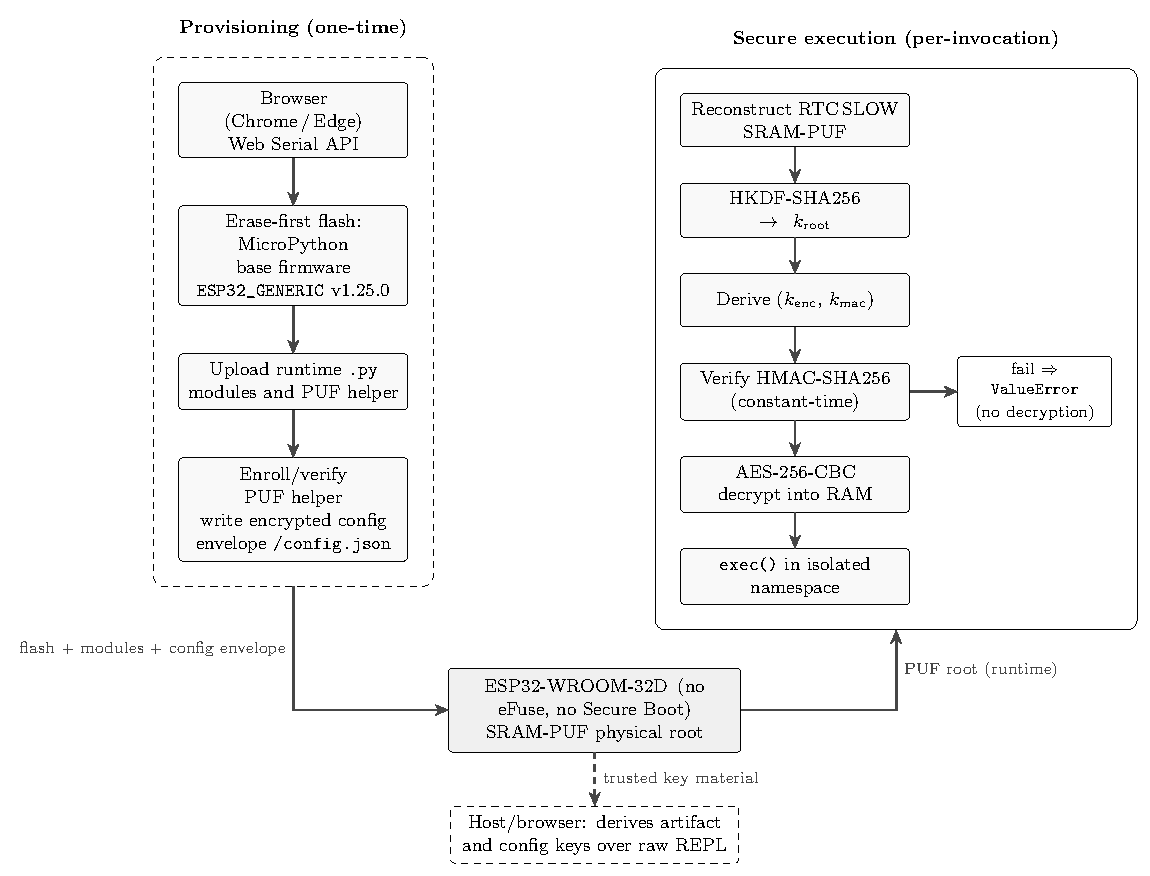
\includegraphics[width=\linewidth]{fig_architecture}
\caption{ROTP-PUF-FLASHER system overview. Left (dashed): one-time provisioning via browser Web Serial, including PUF-helper enrollment and encrypted configuration injection. Right (solid): per-invocation PUF-bound encrypted MicroPython execution. The trusted host/browser derives artifact and configuration keys over raw REPL; the device independently reconstructs them from the enrolled helper at runtime.} \label{fig:architecture}
\end{figure}

\subsection{Design Principles}

Three principles govern the design.

\begin{description}
\item[Reversibility.] No eFuse is burned; no irreversible hardware change is made. The device can be re-enrolled, re-flashed, or re-purposed.

\item[Standard primitives only.] AES-256-CBC~\cite{nist2023fips197} and SHA-256 are used via MicroPython's built-in \texttt{ucryptolib} and \texttt{uhashlib}; HMAC-SHA256~\cite{krawczyk1997hmac} and HKDF-SHA256~\cite{krawczyk2010hkdf} are local RFC-compliant constructions over SHA-256. No proprietary or custom cryptographic primitives are introduced.

\item[Fail-closed.] The loader verifies the HMAC tag before any decryption. If verification fails, the encrypted module is not executed and no plaintext is produced.
\end{description}

\subsection{Component Overview}

Figure~\ref{fig:architecture} shows the end-to-end flow. The provisioning phase (dashed box, left) runs once at device setup, entirely from the browser over Web Serial (detailed in Sect.~\ref{sec:implementation}). The secure execution phase (solid box, right) runs on every payload invocation: the RTC~SLOW PUF is reconstructed on the MicroPython device, a 32-byte symmetric key is derived, and the AES-256-CBC+HMAC-SHA256 envelope is verified and decrypted into RAM.

\section{Implementation}
\label{sec:implementation}


\subsection{PUF Enrollment and Key Derivation}

Enrollment runs once per device, driven from the host over the raw REPL by the published enrollment scripts. The device samples the RTC~SLOW SRAM region at address \texttt{0x50000000} ($N=1000$, $s=4096$\,bytes per sample) using register cycling to expose unstable transient values, with a 50\,ms power-off interval between samples that minimizes reconstruction noise (Sect.~\ref{sec:performance}). It then selects 256 stable bits with a distributed-window policy (64 windows, 128 candidates per window) and protects them with a repetition-8 error-correcting code. These 256 selected, error-corrected bits feed HKDF-SHA256 to back the AES-256 key; their effective entropy is bounded by the selection policy and is not formally quantified here. The 32-bit selection from earlier memory-constrained trials is not a security configuration. Helper data (selected positions, ECC data, salt, context, mode) are stored in the ESP32 non-volatile storage (NVS) under namespace \texttt{rtc\_puf} with a filesystem fallback at \texttt{/puf\_helper.bin}.

Identity reconstruction for key derivation (\texttt{rtc\_slow\_puf\_native.derive\_key}) takes $A=5$ voting attempts over fresh PUF samples, applies vote-majority reconstruction, and feeds the consensus material into HKDF-SHA256~\cite{krawczyk2010hkdf}:

\begin{equation}
\begin{array}{l}
k_{\mathrm{root}} = \mathrm{HKDF}\mbox{-}\mathrm{SHA256}\bigl(
  \mathit{material},\;
  \mbox{\texttt{"DID-PUF-RTC-SLOW-v1"}},\\
\hfill
  \mbox{\texttt{"puf\_identity\_key"}} \,\|\, \mathit{nonce},\;
  32\bigr),
\end{array}
\label{eq:kdf}
\end{equation}

\noindent with arguments in the order (input keying material, salt, info, output length), here and in Eq.~\ref{eq:subkeys}; $\|$ denotes concatenation, and a null-byte separator (\texttt{\textbackslash x00}) is inserted by \texttt{\_info\_bytes()} between the context and nonce strings. No key material is stored persistently; it is reconstructed from the PUF on each invocation.

\subsection{Encrypted Firmware Envelope}

The host tool \texttt{build\_encrypted\_firmware\_from\_device.py} fetches $k_{\mathrm{root}}$ from the device over the raw REPL, keeps it in host RAM, and derives two independent subkeys:

\begin{equation}
\begin{array}{l}
(k_{\mathrm{enc}}, k_{\mathrm{mac}}) =
  \mathrm{HKDF}\mbox{-}\mathrm{SHA256}\bigl(
  k_{\mathrm{root}},\;
  \mbox{\texttt{"DID-PUF-FIRMWARE-ENVELOPE-v1"}},\\
\hfill
  \mbox{\texttt{"aes-256-cbc+hmac-sha256"}},\;
  64\bigr).
\end{array}
\label{eq:subkeys}
\end{equation}

The envelope format \texttt{PUFENC1} is:

\begin{center}
\begin{tabular}{lll}
\toprule
Field & Size & Description \\
\midrule
Magic    & 8\,B  & \texttt{PUFENC1\textbackslash 0} \\
Version  & 1\,B  & Currently 1 \\
Reserved & 3\,B  & Zero \\
IV       & 16\,B & Random initialization vector \\
Length   & 4\,B  & Ciphertext length (big-endian) \\
Ciphertext & $\ell$\,B & AES-256-CBC(plaintext, $k_{\mathrm{enc}}$, IV) \\
Tag      & 32\,B & HMAC-SHA256($k_{\mathrm{mac}}$, header $\|$ ciphertext) \\
\bottomrule
\end{tabular}
\end{center}

\noindent Total header overhead is 32\,bytes; total envelope overhead is $32 + 32 + \mathrm{padding} = 64{+}$\,bytes (65--80\,bytes depending on the plaintext length modulo the AES block size). Measured on a 587-byte \texttt{protected\_app.py} build: a 656-byte envelope ($+69$\,bytes, 11.75\%).

\subsection{Secure Loader and Execution}

The loader (\texttt{secure\_firmware\_loader.py}) remains in cleartext on the device. Its execution path implements a strict \emph{verify-before-decrypt} policy:

\begin{enumerate}
\item Reconstruct the PUF and derive $k_{\mathrm{root}}$ via \texttt{derive\_key()}.
\item Derive $(k_{\mathrm{enc}}, k_{\mathrm{mac}})$ from $k_{\mathrm{root}}$ (Eq.~\ref{eq:subkeys}).
\item Read the encrypted envelope from \texttt{protected\_app.enc}.
\item Parse and validate the \texttt{PUFENC1} header.
\item Compute the expected HMAC-SHA256 tag over \texttt{header $\|$ ciphertext}.
\item Compare tags in constant time (\texttt{\_constant\_time\_equal}).
\item \textbf{If the tag does not match, raise \texttt{ValueError}; execution halts.}
\item Decrypt with AES-256-CBC and remove PKCS\#7 padding.
\item Execute the plaintext module in an isolated namespace via \texttt{exec()}.
\end{enumerate}

\noindent For the \texttt{.mpy} bytecode path, the decrypted bytes are written to a temporary root-level file, imported once, and then deleted from both the filesystem and \texttt{sys.modules} in a \texttt{finally} block.

\subsection{Browser-Based Provisioning}

The Web Flasher uses the Web Serial API (Chrome and Edge) to provision the MicroPython runtime end-to-end from the browser. It flashes the MicroPython base firmware (\texttt{ESP32\_GENERIC-20250415-v1.25.0.bin}) with an erase-first policy, uploads the runtime \texttt{.py} modules as text through the raw REPL, enrolls the runtime PUF helper when absent, derives a configuration key with nonce \texttt{config-json-v1}, and stores \texttt{config.json} as an authenticated AES-256-CBC+HMAC-SHA256 envelope:

\begin{lstlisting}[caption={Plaintext configuration fields encrypted before storage.}]
{
  "device_id":  <integer id>,
  "api_key":    "<API credential>",
  "device_key_hex": "<64 hex chars>",
  "server_key_hex": "<64 hex chars>",
  "server_url": "http://<server-ip>",
  "server_port": 8000,
  "wifi_ssid":  "<2.4GHz SSID>",
  "wifi_pass":  "<password>",
  "read_interval_s": 30,
  "location":   "<deployment label>"
}
\end{lstlisting}

\noindent The tool also scans Wi-Fi networks, offers a filtering serial monitor with exportable logs, manages device files, and generates a provisioning report for laboratory tracking. A hardware smoke test on an ESP32-WROOM-32D exercised the browser base-image flash, runtime-module upload, encrypted \texttt{config.json} deployment, reboot-load, tamper rejection, plaintext-config rejection, and final restore. A heap-collection fix then allowed Wi-Fi activation, NTP synchronization, backend puzzle authentication (HTTP~200), token acquisition, and four telemetry cycles accepted by the server (HTTP~201), confirmed by MongoDB readings and Redis session state.

\medskip
\noindent\textbf{Scope note.} The Web Flasher handles MicroPython runtime provisioning only (base firmware flash, module upload, PUF-helper enrollment, and encrypted configuration injection). Encrypted payload build and secure execution remain separate from the browser tool. Raw REPL uploads are text-based; binary PUFENC1 envelopes remain a CLI-operated step. The encrypted \texttt{config.json} protects configuration at rest against passive flash reads, but not against physical loader replacement without Secure Boot (Sect.~\ref{sec:discussion}).

\subsection{Update Delivery Scope}

The prototype protects modules after they are provisioned, but it does not claim a complete software-update mechanism. Authenticated remote delivery, versioned manifests, transport security, and server-side admission remain future work.


\section{Security Evaluation}
\label{sec:security}


We evaluate ROTP-PUF-FLASHER against three complementary security frameworks. OWASP IoT Top~10 is a practitioner checklist rather than a formally peer-reviewed standard; we use it as a structured framing tool alongside the normative NIST IR~8259A baseline and the STRIDE methodology. Each row carries an evidence label: \textbf{P}~(prototype, lab control), \textbf{Prop}~(proposed, not yet implemented), \textbf{B}~(blocked by design constraint); -- marks out-of-scope categories; combined labels apply per sub-mechanism. Rows marked $^*$ share the open problem that the decryption key depends on the PUF alone (Sect.~\ref{sec:discussion}).

\subsection{OWASP IoT Top 10}

Table~\ref{tab:owasp} maps each OWASP IoT Top~10 category to the corresponding security mechanism in ROTP-PUF-FLASHER.

\begin{table}[ht]
\caption{OWASP IoT Top~10 (2018) mapping.}
\label{tab:owasp}
\centering
\setlength{\tabcolsep}{3pt}
\begin{tabularx}{\linewidth}{llXl}
\toprule
\# & Category & How addressed & Status \\
\midrule
I1 & Weak/Hardcoded Passwords
   & Credentials injected at provisioning, not hardcoded in firmware; \texttt{config.json} stored as a PUF-bound envelope (I7)
   & \textbf{P} \\
I2 & Insecure Network Services
   & Outside this scope; provisioning reduces endpoint exposure
   & -- \\
I3 & Insecure Ecosystem Interfaces
   & Web Serial local interface; no exposed cloud API
   & \textbf{P} \\
I4 & Lack of Secure Update
   & Not addressed by the current paper; authenticated update delivery remains future work
   & -- \\
I5 & Insecure/Outdated Components
   & Standard current primitives; pinned MicroPython v1.25.0 base image; no formal vulnerability-management process
   & \textbf{P} \\
I6 & Insufficient Privacy Protection
   & Not addressed in this scope
   & -- \\
I7 & Insecure Data Transfer/Storage
   & Protected module ciphertext and PUF-bound \texttt{config.json} envelope on flash; plaintext exists in RAM/browser during use
   & \textbf{P}$^*$ \\
I8 & Lack of Device Management
   & Demo backend authentication observed; lifecycle/admission remains future work
   & \textbf{Prop} \\
I9 & Insecure Default Settings
   & Provisioning requires explicit configuration; loader fail-closed on HMAC failure
   & \textbf{P} \\
I10 & Lack of Physical Hardening
   & Reversible design excludes eFuses; physical loader replacement not prevented
   & \textbf{B} \\
\bottomrule
\end{tabularx}
\end{table}

\subsection{NIST IR~8259A Baseline}

Table~\ref{tab:nist} evaluates the tool against the six core device cybersecurity capabilities defined in NIST IR~8259A.

\begin{table}[ht]
\caption{NIST IR~8259A core device cybersecurity capability baseline.}
\label{tab:nist}
\centering
\setlength{\tabcolsep}{3pt}
\begin{tabularx}{\linewidth}{lXl}
\toprule
Capability & How addressed & Status \\
\midrule
Device Identification
  & PUF-reconstructed identity from silicon; three-board uniqueness evidence; backend puzzle authentication observed
  & \textbf{P} \\
Device Configuration
  & \texttt{config.json} encrypted from the browser and written atomically; Wi-Fi scan-assisted selection
  & \textbf{P}$^*$ \\
Data Protection
  & Protected module ciphertext on flash; PUF-bound configuration envelope; plaintext confined to runtime paths
  & \textbf{P}$^*$ \\
Logical Access to Interfaces
  & Web Serial local; no exposed network service during provisioning
  & \textbf{P} \\
Software Update
  & Not implemented in this paper; authenticated remote update delivery is future work
  & \textbf{Prop} \\
Cybersecurity State Awareness
  & Lifecycle/admission states proposed; audit logs are future work
  & \textbf{Prop} \\
\bottomrule
\end{tabularx}
\end{table}

\subsection{STRIDE Threat Analysis}

Table~\ref{tab:stride} analyzes each STRIDE threat category against the provisioning and secure execution flow.

\begin{table}[ht]
\caption{STRIDE analysis of the provisioning and secure execution flow.}
\label{tab:stride}
\centering
\setlength{\tabcolsep}{3pt}
\begin{tabularx}{\linewidth}{lXl}
\toprule
Threat & Mechanism and evidence & Status \\
\midrule
Spoofing
  & PUF-bound configuration plus backend puzzle authentication; server-mediated key origin still future work
  & \textbf{P}$^*$ \\
Tampering
  & HMAC-SHA256 verified in constant time before any decryption; tamper rejection measured at 2.46\,s
  & \textbf{P} \\
Repudiation
  & Not addressed; append-only lifecycle log is future work
  & -- \\
Information Disclosure
  & Passive flash reads expose module/config ciphertext; loader replacement can still expose runtime material
  & \textbf{P}$^*$ \\
Denial of Service
  & Not addressed in this scope
  & -- \\
Elevation of Privilege
  & Boot-path integrity is blocked without Secure Boot; server-mediated key origin remains future work
  & \textbf{B}/\textbf{Prop} \\
\bottomrule
\end{tabularx}
\end{table}

\subsection{Adversarial Test Results}

The demo check script (\texttt{run\_encrypted\_mpy\_demo\_check.py}) runs a
positive control and a tamper case on the enrolled device (a restored-positive
control confirms recovery); timings were taken at the host
(Sect.~\ref{sec:performance}). Table~\ref{tab:adversarial} summarizes the two timed cases.

\begin{table}[ht]
\caption{Adversarial test results on ESP32-WROOM-32D; both cases ran sequentially on the same enrolled device.}
\label{tab:adversarial}
\centering
\begin{tabular}{lll}
\toprule
Case & Result & Time (s) \\
\midrule
Positive (own PUF key)
  & \texttt{PROTECTED\_APP\_MPY\_OK}
  & 2.47 \\
Tamper (1-byte XOR flip)
  & \texttt{HMAC verification failed}
  & 2.46 \\
\bottomrule
\end{tabular}
\end{table}

\noindent The tamper case confirmed fail-closed behavior on the real board: the loader raised \texttt{ValueError} before any decryption began. Tamper rejection (2.46\,s) costs essentially the same as successful execution (2.47\,s): both reconstruct the PUF first, and that reconstruction dominates the runtime, so the security property here is \emph{verify-before-decrypt} correctness, not a timing advantage. Cross-device and wrong-PUF-helper replay were also exercised and rejected in every tested direction across three boards (Sect.~\ref{sec:performance}). The remaining adversarial gap is a downgrade test, pending the monotonic version counter discussed in Sect.~\ref{sec:discussion}.


\section{Performance Evaluation}
\label{sec:performance}

All timing measurements were taken on board A, an ESP32-WROOM-32D (ESP32-D0WD-V3, 240\,MHz, 520\,KB SRAM) running the MicroPython v1.25.0 base image of Sect.~\ref{sec:implementation}, connected via USB-serial; the PUF quality characterization extends to three boards. Timing was measured end-to-end at the host using Python's \texttt{time.monotonic()} across the full serial round-trip including file upload and REPL execution.

\subsection{Timing Measurements}

Table~\ref{tab:timing} summarizes the measured costs.

\begin{table}[ht]
\caption{Performance on ESP32-WROOM-32D, MicroPython v1.25.0. Per-operation times are medians of five runs (variation under 1\%, apart from a higher cold-start reconstruction); enrollment is from its one-time setup log and is excluded from per-invocation cost. Wall-clock times include USB-serial latency and are independently rounded.}
\label{tab:timing}
\centering
\begin{tabularx}{\linewidth}{l r >{\raggedright\arraybackslash}X}
\toprule
Operation & Time (s) & Notes \\
\midrule
PUF enrollment (setup only) & 445.9
  & 1000 samples, 256 bits, size $=$ 4096\,B; not per-boot \\
\midrule
PUF identity reconstruction & 2.23
  & $A=5$ vote-majority attempts; zero bit errors \\
Envelope build (pure crypto)  & 0.01
  & AES-256-CBC + HMAC-SHA256 over 587\,B; host-only \\
Envelope build (total)        & 7.53
  & Includes device round-trips for key derivation \\
Secure firmware execution      & 2.47
  & PUF recon + HMAC verify + AES decrypt + exec in RAM (\texttt{.py} path) \\
Tamper rejection               & 2.46
  & HMAC fails before decryption; fail-closed \\
\midrule
Envelope overhead & $+69$\,B (11.75\%)
  & 587\,B plaintext $\to$ 656\,B envelope \\
\bottomrule
\end{tabularx}
\end{table}

The end-to-end build (7.53\,s) is dominated by device round-trips for key derivation (7.52\,s), not by the cryptographic computation (0.01\,s); the host tool performs several device-side reconstructions in one raw-REPL session, and consolidating them would bring the build close to the per-invocation cost (about 2.2\,s).

\subsection{PUF Quality Under Lab Conditions}

We characterized the PUF on three ESP32-D0WD-V3 boards in the complete configuration (Table~\ref{tab:puf_quality}): boards A and B are WROOM-32D modules; board C is a D1~R32 module (same silicon, different form factor and USB-serial bridge).

\begin{table}[ht]
\caption{PUF reconstruction quality on three ESP32-D0WD-V3 boards (A, B: WROOM-32D; C: D1~R32), complete configuration. Percentages are over the 10\,240 bits sampled per reconstruction (2048 helper positions, five voting attempts). Worst-case post-ECC error stays far below the native bar (0.15\%) and the 5\% policy; reconstruction was accepted on every trial.}
\label{tab:puf_quality}
\centering
\begin{tabular}{lrrr}
\toprule
Metric & Board A & Board B & Board C \\
\midrule
Same-boot worst error (post-ECC) & 0.0098\% & 0.0098\% & 0.0098\% \\
Post-reset worst error (post-ECC) & 0.0098\% & 0.0684\% & 0.0391\% \\
Uniformity (Hamming weight) & 50.2\% & 50.0\% & 49.5\% \\
\bottomrule
\end{tabular}
\end{table}

\noindent Reconstruction is stable on all three boards: the worst same-boot post-ECC error is a single corrected bit (0.0098\%) on each, and reconstruction was accepted on every same-boot, reset, and physical power-cycle trial, always yielding the same per-device key (ten same-boot and eight hardware-reset reconstructions per board, plus two physical USB power cycles with four reconstructions each on boards A and B). Inter-device uniqueness is near the 50\% ideal (raw inter-chip Hamming distance 49.19\% A--B, 49.74\% A--C, 49.86\% B--C), and cross-device replay was rejected in all five tested directions (another board's helper gives ${\approx}$36\% error, \texttt{accepted=False}, no key), so a stolen helper does not reconstruct the key elsewhere. These are nominal room-temperature results for the MicroPython RTC~SLOW PUF (the laboratory control of Sect.~\ref{sec:discussion}): temperature, voltage, aging, and a larger population remain future work. Enrollment used a 50\,ms power-off interval; the loader reconstructs at the default 10\,ms and tolerates the mismatch (worst error 0.0195\%, zero residual errors). The complete configuration enrolls with ${\approx}$128\,KB of free heap; a tighter setup (${\approx}$108\,KB) instead raised a \texttt{MemoryError}, a setup-dependent limit, not a property of the algorithm.


\section{Discussion and Limitations}
\label{sec:discussion}


\paragraph{Central Open Problem: Key Depends on the PUF Alone.}
The decryption key $k_{\mathrm{root}}$ is derived exclusively from the PUF response (Eq.~\ref{eq:kdf}). An adversary who reconstructs the PUF (feasible without Secure Boot) obtains the same key and can decrypt the protected modules. Furthermore, the host obtains $k_{\mathrm{root}}$ over the raw REPL to build the payload, and the browser obtains derived configuration-key material during provisioning, so both are trusted parties in the current architecture. The architecturally correct solution is server-mediated key and configuration origin, with the server participating in key generation and releasing operational configuration only after online authentication; this central thesis extension is reserved for future publication.

\paragraph{MicroPython Is a Laboratory Control.}
The RTC~SLOW adaptation does not claim equivalence with the native \texttt{esp32\_puflib}; the Python loader is a research prototype, not a production security mechanism. The symmetric construction is standard and the 256-bit selection backs a nominally full-strength key (a formal entropy analysis is pending), but production use still needs per-build nonces with rollback protection (a fixed nonce leaves old envelopes replayable until a monotonic version counter is added), key-buffer zeroization, an envelope size cap, server-side payload signing independent of the PUF key, and host handling that never exposes the root key; the demonstrated \texttt{.py} path (RAM-only) is preferred over the \texttt{.mpy} path, which briefly writes plaintext to disk.

\paragraph{Web Flasher Hardware Smoke and Backend E2E.}
The hardware smoke and backend exercise of Sect.~\ref{sec:implementation} surfaced two practical issues: a heap shortage that initially blocked Wi-Fi driver activation (fixed with explicit garbage collection before Wi-Fi initialization) and an encrypted-configuration server key that had to be realigned with the selected FastAPI backend. After both fixes, the device completed puzzle authentication, received a token, sent temperature and humidity telemetry, and the server accepted the readings with HTTP~201 while preserving an active Redis session.

\paragraph{No Secure Boot or Flash Encryption.}
Without Secure Boot, an attacker with physical write access can replace the loader itself, bypassing all encryption checks and extracting PUF-derived material at runtime. Without Flash Encryption, public code, helper data, and ciphertext envelopes remain readable from flash; the protected module and \texttt{config.json} remain ciphertext under passive extraction, but not under active boot-path replacement. These are intentional limits of the reversible, no-eFuse line, not oversights.

\section{Conclusion and Future Work}
\label{sec:conclusion}

We presented ROTP-PUF-FLASHER, a tool integrating browser-based controlled provisioning, PUF-bound encrypted configuration storage, and PUF-bound encrypted MicroPython firmware execution for ESP32-class IoT devices, evaluated against OWASP IoT Top~10, NIST IR~8259A, and STRIDE. On a real ESP32-WROOM-32D board the per-invocation operations complete in about 2.5\,s with a $+69$-byte (11.75\%) firmware-envelope overhead, the fail-closed loader rejects a single-byte tamper before decryption, the Web Flasher path reaches backend puzzle authentication and accepted telemetry (repeated three consecutive times on two WROOM-32D boards), and the PUF was characterized across three boards (inter-device Hamming distance near 50\%, cross-device rejection in every tested direction). Prior work covers the surrounding threads separately; among the surveyed works, none combines browser-based provisioning with PUF-bound encrypted execution or applies these three frameworks simultaneously to a PUF implementation on commodity ESP32 hardware.

The central open problem, that key material still depends on the PUF and is exposed to a trusted host or browser during artifact construction, is stated explicitly and deferred to the thesis. Future work includes server-mediated key and configuration origin via authenticated key exchange, a lifecycle/admission server with revocation, authenticated remote OTA with TLS and signed manifests, post-quantum manifest signatures, and environmental PUF characterization over a larger board population.

\medskip
\noindent\textbf{Reproducibility.}
Source code, measurement scripts, pre-compiled binaries, and documentation: \url{https://github.com/agustinra24/rotp-puf-flasher-congreso}.

\begin{credits}
\subsubsection{\ackname} The authors thank INAOE's Master's program in Security Science and Technology for the laboratory infrastructure.

\subsubsection{\discintname} R.C.~Campos S\'anchez coauthored the prior work cited as~\cite{salinas2026ejecucion}; the authors have no other competing interests relevant to this article.
\end{credits}

\bibliographystyle{splncs04}
\bibliography{references}

\end{document}
